\documentclass[12pt,a4paper]{report}
\pagestyle{empty}
\usepackage{amsmath}
%\usepackage[utf8]{inputenc}
\usepackage{fancyhdr}
\usepackage{graphicx}
\usepackage{booktabs}
\usepackage{array}
\bibliographystyle{ieeetr}
\usepackage{float}
\usepackage{xcolor}
\usepackage{caption}
\usepackage{lipsum}
\usepackage{subcaption}
%\usepackage[demo]{graphicx}
%\usepackage{babel,blindtext}
\usepackage{graphicx}
\usepackage[top=.9in, bottom=.9in, left=1.5in, right=.8in]{geometry}
\usepackage[font=small,labelfont=bf]{caption}
\usepackage{float}
\usepackage{listings}

\renewcommand{\baselinestretch}{1.5} 
\floatstyle{plaintop}
\restylefloat{table}
\newcommand\Fontvi{\fontsize{8}{10.2}\selectfont}
\usepackage{sidecap}
\usepackage{hyperref}
\hypersetup{
    colorlinks=true, %set true if you want colored links
    linktoc=all,     %set to all if you want both sections and subsections linked
    linkcolor=black,  %choose some color if you want links to stand out
	citecolor=black %http://tex.stackexchange.com/questions/50747/options-for-appearance-of-links-in-hyperref
}
\restylefloat{table}
\begin{document}
\begin{center}
        \centering
        \large \textbf{EVALUATION OF WEB SECURITY MECHANISMS
        	USING VULNERABILITY ANALYSIS \& PATTERN MINING }\\[0.3cm]
        \large \textbf{MAINPROJECT PHASE 1 REPORT }\\[.25cm]
         \textit{Submitted By} \\ [0.2cm]
        \bfseries{BIMAL VARGHESES} \\[.4cm]
         \small{\textit{Under The Guidance Of}} \\ [0.2cm]
         \large \textbf{{Ms. SIMI STEPHEN}} \\[.3cm]
        \small{\textit{in partial fulfillment of the requirements for the award of the degree of}}\\[.6cm]
        \large{\bfseries MASTER OF TECHNOLOGY}\\[0.3cm]
        \small{\textit{in}}\\[0.3cm]
        \large{\bfseries COMPUTER SCIENCE AND ENGINEERING\\
        (SPECIALIZATION IN INFORMATION SYSTEMS)}
         \\[.5cm]
    
\includegraphics[scale=1.1]{fisat.jpg}\\[.5\baselineskip]
           
        \large \bfseries{FEDERAL INSTITUTE OF SCIENCE AND TECHNOLOGY (FISAT)}\\
        \small \bfseries{ANGAMALY-683577, ERNAKULAM (DIST)}\\[0.3cm]
        \small {\textit{Affiliated to}}\\[.3cm]
        \large \bfseries{MAHATMA GANDHI UNIVERSITY}\\
        \small \bfseries{Kottayam-686560}\\[.3cm]
        \small \bfseries{April 2015}
       % Word Count: {\color{red}xxxxx}
\end{center}       




















\begin{center}
\renewcommand{\baselinestretch}{1.5} 
 \textbf{FEDERAL INSTITUTE OF SCIENCE AND TECHNOLOGY}\\
 \textbf{(ANGAMALY, ERNAKULAM-683577)}\\[2\baselineskip]
  
\includegraphics[scale=1.1] {fisat.jpg} \\[2\baselineskip]
 \underline{\textbf{CERTIFICATE}} \\[2\baselineskip]
 \end{center}
\vspace{1cm}
This is to certify that this main project phase 1 report  entitled \textbf{``EVALUATION OF WEB SECURITY MECHANISMS
	USING VULNERABILITY ANALYSIS \& PATTERN MINING''} by $ $ $  $ \textbf{BIMAL VARGHESE (82904)},  submitted in partial fulfilment of the requirements for the award of the degree of Master of Technology in Computer Science and Engineering (Specialization in Information Systems) of Mahatma Gandhi University, Kottayam during the academic year 2014-15, is a bonafide record of work carried out under our guidance and supervision.
\\\\\\\\
\textbf{Project Guide:}\hspace*{7cm}\textbf{Head Of The Department}\\
%\vspace*{2mm}
\small{Ms.Simi Stephen}\\
\small{Asistant Professor}\\
\small{Department of Computer Science and Engineering }\\
\small{FISAT}\\
 

\begin{center}
 \textbf{FEDERAL INSTITUTE OF SCIENCE AND TECHNOLOGY}\\
 \textbf{(FISAT)}\\[1\baselineskip]
 {DEPARTMENT OF COMPUTER SCIENCE \& ENGINEERING}\\[2cm]
 
\includegraphics[scale=1.1] {fisat.jpg} \\[2\baselineskip]
 \underline{\textbf{DECLARATION OF ORIGINALITY OF WORK}} \\[2\baselineskip]
 \end{center}
\vspace{1.5cm}
I, \textbf{BIMAL VARGHESE} ,University Reg. No. \textbf{82904}, student of \textbf{M.Tech CSIS 2013-2015}, hereby declare that the project work entitled \textbf{``EVALUATION OF WEB SECURITY MECHANISMS
	USING VULNERABILITY ANALYSIS \& PATTERN MINING''} is an original one and has neither been submitted earlier to this institution nor submitted by me to any other institution for fulfillment of the requirement of a course of study.
.\\\\\\
Name of the student: \textbf{BIMAL VARGHESE}\\
University Reg num: \textbf{82904}\\
Sem,Branch, Course: \textbf{III,CSIS,M.Tech}
\\
%\end{center} 
 \pagenumbering{roman}
    \setcounter{page}{4} 
\addcontentsline{toc}{chapter}{\bf ACKNOWLEDGEMENT}     

    {\centering
    {\large \textbf{\underline{ACKNOWLEDGEMENT}}}
     %{\rule{3 cm}{1 pt}}
    \\[4\baselineskip]}
    {Initially, I would like to thank, the God Almighty for showering his blessings on me for successful completion of this mainproject phase 1 report.\\[.4cm]
I extend my gratitude to the Principal of FISAT \textbf{Dr. C. Sheela} who supported me for the success of this project.\\[.4cm]
I would also like to thank from the bottom of my heart, Head of the Department of Computer Science \& Engineering, \textbf{Dr. Prasad J C} for encouraging me.\\[.4cm]
I would like to thank my internal guide \textbf{Ms. SIMI STEPHEN} for her relentless support and encouragement.\\[.4cm]
I would like to thank all the teachers in the panel for their valuable support. It
would be never have been possible for me to take this project to this level
without their support and encouragement.
 }\\[4\baselineskip]
        
    %\begin{minipage}{.5\textwidth}
    \begin{flushright}
    \bf BIMAL VARGHESE\\
    \end{flushright}
  %\end{minipage} 
\addcontentsline{toc}{chapter}{\bf ABSTRACT} 
 %\pagenumbering{roman}
  %  \setcounter{page}{4}
{\centering
        
        {\large \textbf{\underline{ABSTRACT}}}
        %{\rule{5 cm}{1 pt}} 
        \\[4\baselineskip]
        }
        %\begin{abstract}
        {\normalsize Internet and web applications have become very common these days. Web applications are accessible by anyone from any part of the world and hence is prone to more attacks. Due to limited time and resources, web application engineers need support in identifying vulnerable code which can be utilized for attacks. A practical approach to predicting vulnerable code would enable them to prioritize security auditing efforts. To evaluate web application security mechanism, a methodology and a prototype tool is proposed. The
       	methodology is based on the idea that injecting realistic vulnerabilities utilizing pattern matching in a web application and attacking them automatically can be
       	used to support the assessment of existing security mechanisms and tools in custom setup scenarios. The system tries to evaluate applications utilizing vulnerabilities in real web applications.
       	In addition to the generic methodology, the paper proposes the implementation of the Vulnerability \& Attack Injector Tool (VAIT) that
       	allows the automation of the entire process.
        	

        } 
\hypertarget{contents}{}
\tableofcontents
\listoftables
\addcontentsline{toc}{chapter}{\bf LIST OF TABLES}
\listoffigures
\addcontentsline{toc}{chapter}{\bf LIST OF FIGURES}


\clearpage
\pagebreak
\pagestyle{fancy}
\lhead{\small {Evaluation Of Web Security Mechanisms Using Vulnerability Analysis \& Pattern Mining}}
\chead{}
\rhead{}
\lfoot{\small {Department of Computer Science and Engineering, FISAT}}
\cfoot{}
\rfoot{\small {\thepage}}
\renewcommand\headrulewidth{0.4pt}
\renewcommand\footrulewidth{0.4pt}


\pagenumbering{arabic}
\setcounter{page}{1}
\chapter{INTRODUCTION}\label{chp:chapter1}
\thispagestyle{fancy}
Web applications are becoming common these days.The users of web 
application range from individuals to organizations and corporate users.
Web applications plays an important role in many of our daily activities such as social networking, email, banking, shopping,
registrations etc.Since a web applications accessibility is very high, the impact of vulnerability in it will also increase dramatically compared to a normal software.Since web applications have huge number of users compared to that of other applications, it becomes a high potential target for attackers.
\\
\newline
Developers of the web applications are having the direct responsibility for the security of web applications.But due to heavy pressure to meet the deadline or lack of knowledge or experience and time constraint limits developers focus on security issues of web applications. A web developer must have a thorough understanding about the magnitude and relevance of the assets they are supposed to protect. Some common reasons why securing a web application become a tricky are 1)availability of a number of frameworks and languages for the development 2)exposure to large number of audience 3)inexperience of developers and 4)need for accessing organizational resources remotely.  \\ 
\newline
So in order to secure a web application, their is a need to have security standards and tools to evaluate the security of them. Also the necessary counter measures have to be taken against the detected attacks. For implementing this, new tools and procedures must be developed and a proper training must be conducted in accordance with them.The testing procedures must be thorough and the application must be verified and validated.The existing legacy applications must be audited from time to time and must be patched or updated timely.\\
\newline
In order to test and validate the security mechanism of web applications a methodology and a tool to inject vulnerabilities and attack the web applications is proposed.The methodology is based on the idea that, it is possible to assess different attributes of existing web application security mechanisms by injecting realistic vulnerabilities in a web application and attacking them automatically.The methodology have evolved from the existing fault injection techniques.The set of ``vulnerability'' +
``attack'' represents the space of the ``faults'' injected in a
web application, and the ``intrusion'' is the result of the
successful ``attack'' of a ``vulnerability'' causing the application to enter in an ``error'' state \cite{15}. A vulnerability can be considered as a weakness whose presence do not cause harm by itself but can be utilized for an attack. \\
\newline
 The attack injection consists of the introduction of realistic vulnerabilities that are afterwards
automatically exploited.Vulnerabilities are
considered realistic because they are derived from the
extensive field study on real web application vulnerabilities  \cite{16}, and are injected according to a set
of representative restrictions and rules.The attack injection methodology is based on the
dynamic analysis of information obtained from the runtime monitoring of the web application behavior and of
the interaction with external resources, such as the backend database. This information, complemented with the
static analysis of the source code of the application,
allows the effective injection of vulnerabilities that are
similar to those found in the real world. The
use of both static and dynamic analysis is a key feature
of the methodology that allows increasing the overall performance and effectiveness, as it provides the means to
inject more vulnerabilities that can be successfully
attacked and discarded those that cannot.\\
\newline
This methodology can be applied to various
types of vulnerabilities.The project focus on only some common exploits namely SQL Injection (SQLi), Cross Site Scripting(XSS), Remote Code Execution (RCE) and File Inclusion (FI).These kinds of attacks occur mainly due to improper validation of the input which allows the attacker to manipulate commands.\\
\newline
The proposed methodology provides a practical environment that can be used to test countermeasure mechanisms (such as intrusion detection systems (IDSs), web
application vulnerability scanners, web application firewalls, static code analyzers, etc.), train and evaluate security teams, help estimate security measures (like the
number of vulnerabilities present in the code), among
others. This assessment of security tools can be done
online by executing the attack injector while the security
tool is also running; or offline by injecting a representative set of vulnerabilities that can be used as a testbed for
evaluating a security tool.
The methodology proposed will be implemented in a concrete Vulnerability \& Attack Injector Tool (VAIT) for web
applications. The tool will test on top of widely used applications in two scenarios. The first to evaluate the
effectiveness of the VAIT in generating a large number of
realistic vulnerabilities for the offline assessment of security tools, in particular web application vulnerability
scanners. Second, how it can exploit injected
vulnerabilities to launch attacks, allowing the online evaluation of the effectiveness of the counter measure mechanisms installed in the target system, in particular an
intrusion detection system\\
\newline
The rest of this report is organized as follows. Chapter \ref{chp:chapter2}, presents the literature survey. Chapter \ref{chp:chapter3} describes the proposed methodology and attack injections,   and Chapter \ref{chp:chapter5} summarizes the conclusion of the survey.
%Chapter \ref{chp:chapter4},describes the proposed methods


\chapter{LITERATURE SURVEY}\label{chp:chapter2}
\thispagestyle{fancy}
Fault injection techniques have traditionally been used to
inject physical (i.e., hardware) faults \cite{18} into a complex system.
The method utilizes the use of fault injection for explicitly removing design or implementation faults in a complex fault tolerant system. 
It explicitly aims in reducing, by verification, the presence of faults in the design or implementation. Here faults are injected to uncover potential issues and thus to determine the most appropriate action for improving the system.Compared to a fault injection system, a fault forecast system can use a feedback loop to impact the design of the system.Usually, fault-injection based attempts to validate systems that consist of test sequences where the input patterns (the injected faults) are selected according to fault or error models intending to simulate the consequences of activating real faults. Heavy ion radiation , pin-level fault injection, software-implemented fault injection , failure acceleration, fault injection in simulation models are typical techniques to perform this objective in the context of physical- or software-fault injection experiments. The fault-tolerance algorithms \& mechanisms (FTAM) formalism enables an execution tree to be generated, where each path from the root to
a leaf of the tree is a well-defined formula. The set of well-defined
formulas constitutes a useful framework that fully characterizes the test sequence. The input patterns of the test sequence (fault \& activation domains) then are determined to cover specific structural criteria over the execution tree (activation of proper sets of paths). This provides a framework for generating a functional deterministic test for programs.The main advantage of this system include generation of causing actual hardware faults, which may be close to a realistic fault model.\\
\newline
 The increasing complexity of systems has lead to the replacement of hardware-based techniques by software implemented fault injection (SWIFI), in which hardware faults are
emulated by software eg. Xception \cite{20}. The high complexity and the very high speed of the processors available today make the design of the special
hardware faults techniques very difficult, or even impossible. It is very difficult to control and observe the fault effects inside the processor compared to injecting the actual problem to the hardware. Even the detection of the activated faults is very complex. So to overcome these difficulties, simulation based fault injection has been proposed.
The injection of realistic software faults (i.e., software
bugs) has been absent from fault injection effort for a
long time.In this method, faults are injected into a simulation model of the target system which allows to control the injection experiment. First proposals were based on ad-hoc code
mutations \cite{22}, \cite{23}.Software Implemented Fault Injection techniques
(SWIFI), also known as fault emulation is a common way for alternate implementation of fault injection method.In this method the application execution is interrupted some way and executing some  specific fault injection software code, which emulates hardware faults by inserting errors in different parts of the system such as the processor register, the memory, or in the application code.The main advantages of software fault injection are the low complexity, low development effort, and low cost.In addition,software fault injection tools have increased portability, can be easily expanded (e.g., for new classes of faults), and do not have problems with
physical and electrical interferences which are very common in physical fault injection tools. The disadvantage of these method include fail to inject faults in peripheral devices and unable to check accuracy of address specific logic system if the hardware.In Xception by directly programming the debugging hardware
inside the target processor, system can inject faults with minimum interference with the target application without modifying it.\\
\newline
%[24]
More recent works focus on the injection of representative software faults based on comprehensive field studies on the most common types of software bugs  \cite{4}.The study
shows that a clear predominance of software faults as the root
cause of computer failures .Given the huge complexity of today's software, the weight of
software faults on overall system dependability will tend
to increase. The complete elimination of software defects
during software development process is very difficult to
attain in practice. In addition to well-known technical
difficulties of the software development and testing
process  \cite{5}, practical constraints such as the intense
pressure to shrink time-to-market and cost of software
contribute to the difficulties in assuring 100 percent
defect-free software.So the current scenario in
the computer industry is having systems in which
software defects do exist but no one knows exactly where
they are, when they will reveal themselves, and,the possible consequences of the activation of the software faults. Trend in the software industry toward a
component-oriented development model, compels the software vendors to consider the use of commonly available general-purpose components more and more, which leads to the software products as a collection of small components from a variety of sources. These kinds of software have the problems like when one of the component software behave erroneous, the entire system become faulty and how to estimate this kind of situations.In order to validate a component software system, an approach to inject
residual software faults at the executable code of the targets
in an accurate manner has been proposed \cite{5}.The establishment
of a utilization scenario for the injection of software faults
from the beginning is important to help in identifying the
requirements put on the accurate emulation of software
faults.
The software fault are injected according to the following principle:\\
\newline
Faults are injected in a given component to evaluate the behavior of
the overall system in the presence of that faulty component.This help to have a separation between target component and system under observation.The behavior of the system under the presence of one faulty component is observed.Using this scenario three major uses can be identified 
\begin{enumerate}
	\item Validation of fault-tolerant mechanisms.
	\item Prediction of worst-case scenarios and experimental risk assessment.
	\item Dependability benchmarking.
\end{enumerate}
The realistic emulation of residual software faults by fault injection at the target executable code is much more difficult. In fact, the problem of emulating software faults is intrinsically difficult. Software faults are by nature human-made faults (at the design, implementation, etc.) and it is extremely difficult to model human errors.\\
\newline
Fault injection techniques to assess the security
is a particular case of software fault injection,
focusing on software faults that represent security vulnerabilities.The existence of a vulnerability may not cause
a security hazard, and in many times they can remain dormant for many years until right attack is discovered and applied to exploit that vulnerability.After an intrusion, the system might
or might not fail, depending on the kind of capabilities it
possesses to deal with errors introduced by the attacker.Intrusions would never arise if all vulnerabilities could be eliminated. Vulnerability removal  \cite{7} can be performed both during the development and operational phases. Vulnerability removal in the operational phase helps to identify programming flaws which can later be corrected. It also assists
the discovery of configuration errors and other similar problems and can reduce the accessibility of the attacker by reducing the number of entry points into the system.Nuno Neves et all \cite{7}  presents a tool called AJECT (Attack inJECtion Tool) that can be used for vulnerability detection
and removal. It simulates the behavior of an adversary by injecting attacks against a target system. Then, it observes the execution of the system to determine if the attacks have caused a failure.If a failure occurs then there exist a vulnerability in the system.If a bug is identified, a developer can use a traditional debugging method and can eliminate the presence of it.AJECT targets network servers and local demons.It performs a blackbox testing knowing only the protocol specifications.Experiments with AJECT was conducted with IMAP servers and was able to detect identified bugs in the bug tracking system as well as new bugs which are not yet identified.\\
\newline
%Analysis of field data
Security of Web applications has become increasingly
important in the recent time. Nearly all information systems and business
applications  are now built as web-based
database applications.The exposure of web application to a wide user audience make it more prone to attacks.Hence an existing vulnerability in web application will most probably be uncovered and will be exploited.Traditional defense strategies such as firewalls do not protect against Web application attacks, as these attacks rely
solely on HTTP traffic, which is usually allowed to pass
through firewalls unhindered.In recent years strongly typed languages like Java \cite{10}, has emerged as the language of choice for building large complex Web-based systems mainly due to language safety features that restrict direct memory access and eliminate problems such as buffer overruns.But, however secure the language is, a logical error can cause a vulnerability in the application which can lead to the failure of the system.Software faults can be detected by performing a static analysis to the code \cite{10}. This is a labor intensive job, usually done with automated tools, although they lack the precision of the manual counterpart.\\
\newline
One of the aspects that contribute to security problems
seems to be related to how bad different programming
languages are in terms of propensity for mistakes. Clowes  \cite{9}
discussed common security problems related to the easiness
in programming with PHP and its features, but this affects
many other programming languages. The choice of the type
system (strong or weak) and the type checking (static or
dynamic) of the programming language also affects the
robustness of the software. For example, a strong typed
language with a static type checking can help deliver a safer
application without affecting its performance  \cite{21}. Scholte et
al.  \cite{19} presented an empirical study on a large set of input
validation vulnerabilities developed in six programming
languages. However, that work focused on the relationship
between the specific programming language used and the
vulnerabilities that are commonly reported, not going into
details in what concerns the typical software faults that
originate vulnerabilities.\\
\newline
The use of software code inspections, has been found
to increase software quality and lower software
development costs.Prior studies indicate that
inspections can detect as little as 20\% to as much as
93\% of the total number of defects in a software.
 To improve the software quality  and to help predict software failures, a new
defect classification scheme was proposed in  \cite{13}.Automated software inspection
(ASI) tools are usually utilized as static analysis tools, coding standard
analysis tools, and source code analysis tools.These
tools produce error messages similar to those of a
compiler. However, they identify additional faults, such
as coding standard non-compliance, uncaught runtime
exceptions, security vulnerabilities, redundant code,
division by zero, and memory leaks.ASI tools are intended to identify faults which
allow the software engineers to recode before they
surface more publicly as manual inspections faults or as
test and field failures. the removal of the defects found by the
ASI can allow the labor-intensive manual reviews to be
more efficient and to focus on more complex, functional
and algorithmic defects.\\
\newline
Measuring significance of software vulnerability can done by analyzing the likelihood of vulnerability discovery.So in-order to understand the software security, the vulnerability discovery's model(VDM) is created. Software  security
is  the  ability  of  a  system  to  perform  its  required  functions
without software-caused violations of its explicit or implicit security policy.For a better understanding software security, two natures of software systems are considered.
\begin{enumerate}
	\item \textbf{Engineering nature: }characterizing features like when was a vulnerability introduced, when was it discovered, how is the
	source code of a system changing, etc. This approach employs statistical analysis of
	vulnerabilities that have already been discovered and characteristics of the systems
	in which they were discovered.
	\item \textbf{Economic nature: }characterizing features like what is the auction-ascertained price
	of a previously-unreported vulnerability in a specific system. Entities offer a steadily
	increasing reward for a vulnerability in a system: the first person to report such a
	vulnerability receives the reward. The reward serves as both an incentive to find a
	vulnerability and a measurement of the perceived value of that vulnerability
\end{enumerate} 
  These two approaches provide insight into the number of vulnerabilities in a
  system, the rate at which they are detected, and the difficulty in doing so.Unfortunately neither of the approach can fully provide information on how many vulnerabilities exist in a system.\\
  \newline  
%main paper
The industry uses fuzzing and mutation testing to automate penetration testing of web applications. They rely on web application vulnerability scanner tools that also generate reports compliant with security regulations. Some of the best known of such tools are HP WebInspect, IBM Watchfire AppScan,Acunetix web application security scanner and WebSphinx. In spite of their continuous development, these tools still have many problems related to the high number
of undetected vulnerabilities and high percentage of false positives, as shown by several studies  \cite{8}. To address these problems, it was proposed a method to benchmark these scanners  \cite{8}. The method starts by identifying all the points where each type of bug can be injected, then injecting the bug. Many of these bugs injected are vulnerabilities that can be used to test and
compare the performance of the scanners.\\
\newline
Web applications usually are not monolithic
but consist of several distributed components. During the
development of the use communication protocols and the web
components, different tools and programming languages may
be used.White-box penetration testing tools usually require that all applications are developed
in the same language (e.g., PHP ,Java etc) which is usually not the case in distributed environments.Black-box penetration testing tools are not really effective due to the weaknesses of
the crawling step that misses lots of potential interaction with the user So the use of a model checkers for security analysis was proposed  \cite{11}.A formal model \textbf{M} for the
specification of the System Under Validation (SUV) is  used.  In this case, the vulnerability is injected by
mutating the formal model of the web application.First, the model  mutated to introduce specific
vulnerabilities present in web applications. Then, a model checker outputs attack traces that exploit those vulnerabilities. 
Next, the attack traces are translated into concrete test cases by
using a 2-step mapping. Finally, the tests are executed on the
real system using an automatic procedure that may request the
help of a test expert from time to time. The model is also used to generate test cases that are used to attack the web application in a semi-automatic way.\\
\newline 
In a competitive commercial software market release of softwares must meet the strict deadlines \cite{12}. A companies survival depends on the time at which the software is released to the market.In such a situation the question arise is ``Is the software good enough to release now? ''. An easiest ways to judge whether a program is ready for release is to measure its defect density — the number of defects per
line of code. Suppose the first version of your
product consists  of 100,000 lines
of code. Further suppose that you detected 650
defects prior to the software's release, and that 50
more defects were reported after release. The
software therefore had a lifetime defect count of
700 defects, and a defect density of 7 defects per
1,000 lines of code (KLOC).\\
\newline
 Another simple defect prediction
 technique is to separate defect reports into two
 groups; say Pool A and Pool B, and then track the defects in these two pools separately. The distinction between the pools is arbitrary ie. it is possible to put all the defects discovered on
 Mondays, Wednesdays, and weekends into Pool
 A, and the rest into Pool B. or split the test team down the middle and put each subgroup's reported defects into its own pool. It
 doesn't matter how the group is divided as long as both subgroups operate independently and both
 test the full scope of the product.\\
 \newline
 After grouping, track the number of defects reported
 in each pool and the
 number of defects reported.The number of unique defects reported at any given time is\\
 
 $ Defects_{ unique} = Defects _{A} +  Defects_{ B} - Defects_{ (A+B)} $\\
 
 The number of total defects can then be
 approximated by the simple formula\\

{ $ Defects_{total} = \frac{Defects_{ A} * Defects_{ B}}{Defects_{ (A+B)}} $} \\

The attacker's perspective has also been of some focus in
the literature  \cite{9}, \cite{17}, \cite{23}, but mainly through
empirical data gathered by the authors highlighting social
networking and what could be obtained from attacking
specific vulnerabilities. Some studies analyzed the attacks
from the victim's perspective, including the proposal of a
taxonomy to classify attacks based on their similarities \cite{2}
and the analysis of attack traces from HoneyPots to separate
the attack types \cite{24}. There is, however, a lack of knowledge
about existing exploits and their correlation with the
vulnerabilities.\\
\newline
%Main
The list of possible types of vulnerabilities affecting web
applications is enormous, but XSS and SQLi are at the top of
that list, accounting for 32 percent of the vulnerabilities
observed \cite{3},\cite{6}.\\
\newline An SQLi attack consists of tweaking the input fields of
the webpage (which can be visible or hidden) in order to
alter the query sent to the back-end database. 
SQL injection attacks pose a serious security threat to Web applications \cite{14}: they allow attackers to obtain unrestricted access to the
databases underlying the applications and to the potentially sensitive information these databases contain.This allows
the attacker to retrieve sensible data or even alter database
records.In some cases, attackers can even
use an SQL injection vulnerability to take control of and corrupt the
system that hosts the Web application.SQL injection refers to a class of code-injection attacks in which
data provided by the user is included in an SQL query in such a
way that part of the user’s input is treated as SQL code.By leveraging these vulnerabilities, an attacker can submit SQL commands
directly to the database. These attacks are a serious threat to any
Web application that receives input from users and incorporates it
into SQL queries to an underlying database. Most Web applications
used on the Internet or within enterprise systems work this way and
could therefore be vulnerable to SQL injection.\\
\newline
There are many
types of SQLIAs and countless variations on these basic types. The different types of attacks are generally not performed in isolation; many of them are used together or sequentially, depending
on the specific goals of the attacker. Some representative examples include
\begin{enumerate}
	\item \textbf{Tautologies}: used for Bypassing authentication, identifying injectable parameters, extracting data.
	\item \textbf{Illegal/Logically Incorrect Queries}: used for  Identifying injectable parameters, performing database
	finger-printing, extracting data.
	\item \textbf{Union Query}: used for Bypassing Authentication, extracting data.
	\item \textbf{Piggy-Backed Queries}: used for Extracting data, adding or modifying data, performing denial of service, executing remote commands.
	\item \textbf{Stored Procedures}: used for Performing privilege escalation, performing denial of service, executing remote commands.
	\item \textbf{Inference}: used for Identifying injectable parameters, extracting data,
	determining database schema.
	\item \textbf{Alternate Encodings}: used for Evading detection.
\end{enumerate}
 An SQLi attack can be dormant for a while and
only be triggered by a specific event, such as the periodic
execution of some procedures in the database.
\\
\newline
A XSS attack consists of injecting HTML and/or other
scripting code (usually Javascript) in a vulnerable webpage. It exploits the common utilization of the user input
(without sanitizing it first) as a building part of a webpage.
When this occurs, by tweaking the input, the attacker is
able to change some of its functions, allowing him to take
advantage of users visiting that webpage. This attack
exploits the confidence a user (victim) has on the website,
allowing the attacker to impersonate these users and even
execute other types of attacks such as cross site request
forgery (CSRF)  \cite{1}. The injection of XSS can also be persistent if the malicious string is stored in the back-end database of the web application, therefore potentiating its
malicious effects in a much broader way.Cross-site scripting vulnerabilities date back to 1996 during the early days of the World
Wide Web (Web).Hackers found that when unsuspecting users visited their Web pages they could forcibly
load any Web site (bank, auction, store, Web mail, and so on) into an HTML Frame within
the same browser window.Then using JavaScript, they could cross the boundary between
the two Web sites, and read from one frame into the other.They were able to pilfer usernames and passwords typed into HTML Forms, steal cookies, or compromise any confidential information on the screen.\\
\newline
An  XSS  attack  manipulates  content  of  a  Web  application 
and  trick  users  into  opening  that  page.  A  typical
XSS  attack work as follows:
\begin{enumerate}
	\item Form  on  the  page  asks  user  for  clicking  a  link,  or 
	entering username or password.
	\item  User takes the data submitted by the victim and store it 
	in a database
	\item User displays that data on the screen to other users.
	\item Malicious user submits Script in their form submission, 
	which  performs  an  action  when  other  users  visit  the  page 
	displaying the data they submitted
\end{enumerate}
XSS vulnerabilities can be divided into following types:
\begin{enumerate}
	\item Injection via URL
	\item Injection by exploiting client side code
	\item Injection by exploiting external feed displayed on a website
	\item Injection via permanently displayed data
\end{enumerate}
Cross-site scripting poses severe application risks as the users can unknowingly execute malicious scripts while viewing
dynamically generated pages or content provided by an attacker. An attacker can take over the user session before the
user's session cookie expires. An attacker can connect users to a malicious server of his choice. An attacker who can
convince a user to access a URL supplied by the attacker could cause script or HTML of the attacker's side to be
executed in the user's browser.\\
\newline
A contribution to better understand the most common
vulnerabilities in web applications was presented in a field
study that classified 655 XSS and SQLi security patches of
six widely used Linux, Apache, MySQL and PHP (LAMP)
web applications \cite{16}.When application vulnerabilities are discovered,
software developers correct the problem releasing
application updates or patches. These patches correcting
vulnerabilities were used to understand
which code is responsible for security problems. With
this approach the code which caused security flaws can be classified.\\
For each web application tested, the methodology to
classify the security patches is the following:
\begin{enumerate}
	\item Verification of the patch to confirm if the version of
	the web application is available.
	\item  Analysis of the code with the vulnerability and of the
	code after being patched.
	\item  Classification of each code fix that is found in the
	patch.
	\item  Loop through the previous steps until all available
	patches of the web application are analyzed.
\end{enumerate}
The study only deals  with
code defects and hence only use the Orthogonal Defect Classification (ODC) defect types
that are directly related to the code are considered.These defect types
are: \textbf{Assignment} (errors in code
initialization), \textbf{Checking} (errors in program logic and
validation), \textbf{Interface} (errors interacting among
components), and \textbf{Algorithm} (errors related to the need
of algorithm change without a design change).\\
\newline
Remote Code Execution (RCE) vulnerability refers to an attacker's ability to execute arbitrary program code on a target server. It is caused by user inputs
in security sensitive functions such as file system calls (e.g., $ fwrite $), code execution functions (e.g., $ eval $), command execution
functions (e.g., $ system $), and directory creating functions (e.g., $ mkdir $).
It allows a remote attacker to execute arbitrary code in the system with administrator privileges. It is an extremely risky
vulnerability, which can expose a web site to different attacks, ranging from malicious deletion of data to web page defacing.
The following code depicts an RCE vulnerability.
\begin{lstlisting}
$comments = $_POST['comments'];
$log = fopen('comments.php','a');
fwrite($log,'<br />'.'<br />'.'<center>'.'Comments::'.'<br />'.
		$comments); //remote code execution possibility
\end{lstlisting}
The above code retrieves user comments and logs them without sanitization. This means that an attacker can execute
malicious requests, ranging from simple information gathering using phpinfo() to complex attacks that obtain a shell on the
vulnerable server using $ shell\_exec() $.
Other sensitive PHP functions and operations associated with this vulnerability type include $ header $, $ preg\_replace() $ with ``/e''
modifier on,
\begin{lstlisting}
 fopen, vassert, create_function, unserialize, 
 $_GET['func_name'], and $_GET['argument'].
\end{lstlisting}


File Inclusion vulnerability refers to an attacker’s ability to include a file that originates from a remote (possibly an attacker’s) server or
ability to access/include a local file that is not intended to be accessed without proper authorization. It is caused by user inputs
being part of filenames or the use of un-initialized variables in file operations. Consider the following code:
\begin{lstlisting}
include($_GET['file']); //remote file inclusion possibility
\end{lstlisting}
An attack may conduct a file inclusion attack using the following values:
\begin{lstlisting}
/include.php?file=http://evil.com/malicious.php
\end{lstlisting}
This attack causes the vulnerable PHP program to include and execute a malicious PHP file that may cause dangerous
program behaviors. Similar PHP commands that may cause FI vulnerability includes $ include\_once, require, $ and $ require\_once. $
Moreover, an FI vulnerability may also appear with PHP operations that involve file accesses and file operations in which the
attacker may be able to view restricted files, or even execute malicious commands on the web server that can lead to a full
compromise of the system. For example, consider the following code:
\begin{lstlisting}
$handle = fopen($_GET['newPath'], "r"); 
//local root file access possibility
\end{lstlisting}
In the above case, the input newPath is received from the HTTP GET parameter. An attacker could provide a value like\\
%\begin{lstlisting}
newPath $ \rightarrow $ ``../../../../../etc/passwd\%00.txt'' \\
%\end{lstlisting}
in order to access the password file from the file system. The expression$  ‘dot-dot-slash (../)’ $ instructs the system to go one
directory up. The attacker has to guess how many directories he has to go up to find the user confidential folder on the system, but
this can be easily done by trial and error. This vulnerability is also known as \textit{directory traversal}

\section{ METHOD COMPARISON}

\begin{table}[H]
	\begin{center}
	\caption{Comparison of various vulnerability analysis methods}
	\label{t1}
	\begin{tabular}{ | m{7cm} | m{3cm}| m{3.5cm} | }%  {|c|c|c|}
		\hline \qquad \qquad \textbf{Paper Name}  & \textbf{Method Used} & \textbf{Implemented on} \\ 
		\hline Fault Injection and
		Dependability Evaluation of Fault-Tolerant Systems  & Fault Injection  & Hardware Level \\ 
		\hline Xception: Software Fault Injection and Monitoring in Processor Functional Units & Fault Injection & Software Simulation \\ 
		\hline Emulation of Software Faults:
		 A Field Data Study and a Practical Approach & Bug Injection & Software Components \\ 
		\hline Using Attack Injection to Discover 
		New Vulnerabilities  & Server Software & IMAP \\ 
		\hline Finding Security Vulnerabilities in Java Applications with	Static Analysis & Static Code Analysis & Java \\ 
		\hline Preliminary Results on Using Static Analysis Tools for Software Inspection  & Source Code Analysis & Coding Standard \\ 
		\hline Semi-Automatic Security Testing of  Web
		Applications from a Secure Model  & Modal Analysis & Web Application Model \\ 
		\hline 
		Gauging Software Readiness with Defect Tracking
		 & Defect Density & Software Defects\\
		 \hline
 
	\end{tabular} 
\end{center}
\end{table}






\chapter{METHODOLOGY}\label{chp:chapter3}
\thispagestyle{fancy}
The evaluation methodology is based on the injection of realistic vulnerabilities and the subsequent controlled exploit of those
vulnerabilities in order to attack the system. This provides a practical environment that can be used to test
counter measure mechanisms (such as IDS, web application vulnerability scanners, firewalls, etc.), train and evaluate security teams, estimate security measures (like the
number of vulnerabilities present in the code, in a similar
way to defect seeding  \cite{12}), among others.To obtain a realistic environment, true
to life vulnerabilities will be consider. As mentioned before,
results from a field study presented in [16] that classified
655 XSS and SQLi security patches of six widely used
LAMP web applications are utilized. This data will help to define
where a real vulnerability is usually located in the source
code and what is the piece of code that is responsible for the
presence of such vulnerability.\\
\newline
A typical web application is referenced , with a web front-end and an access to a back-end database to store the dynamic content and business data (Fig. 3.1).The vulnerabilities are injected in the web application following a realistic pattern . The information
about what was injected is fed to the injection mechanism in
order to improve the attack success rate.


\begin{figure} [H]
\centering
\fbox{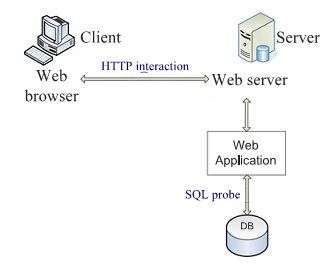
\includegraphics[width=0.65\linewidth]{Main/Fig1}}
\caption{A normal Web Application Setup}
\label{fig:Fig1}
\end{figure}

The attack injection tool uses two external
probes as shown in Fig 3.2: one for the HTTP communication and other for the
database communication.These probes monitor the HTTP
and SQL data exchanged, and send a copy to be analyzed
by the attack injection mechanism.
\begin{figure}[H]
\centering
\fbox{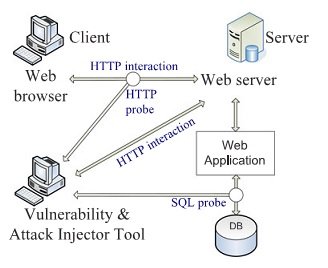
\includegraphics[width=0.7\linewidth]{Main/Fig2}}
\caption{VAIT setup}
\label{fig:Fig2}
\end{figure}

This is a key aspect of
the methodology to obtain the user interaction and the
results produced by such interaction for analysis, so they
can be used to prepare the attack. Therefore, the attack injection mechanism is aware of important inner workings of the
application while it is running. For example, this provides
insights on what piece of information supplied to a HTML
FORM is really used to build the correlated SQL query and
in which part of the query it is going to be inserted.The entire process is performed automatically, without human intervention.\\
\newline
%Example --can be removed if needed
For example,  consider the evaluation of an IDS: during the attack stage, when the IDS
inspects the SQL query sent to the database, the VAIT also
monitors the output of the IDS to identify if the attack has
been detected by the IDS or not. Only the
final results of the attack injection has to be collected, which also contains,the IDS detection output.\\
\section{ATTACK PROCEDURE}
The attack procedure mainly consist of 4 stages
\begin{enumerate}
	\item Preparation stage
	\item Vulnerability injection stage
	\item Attackload generation stage
	\item Attack stage
\end{enumerate}

\subsection{Preparation Stage}
In the preparation stage, the web application is interacted (crawled), executing all the functionalities that need to be tested (Fig.3.3). Both HTTP and SQL communications are captured by the two probes and processed for later use. The interaction with the web application is always done from the client's point of view.The outcome of this stage is the correlation of the input values, the HTTP variables that carry them and their respective source code files, and its use in the structure of the database queries sent to the back-end database (for SQLi) or displayed back to the web browser (for XSS).\\
\newline
Later, in the attack stage, the malicious activity applied is based on tweaking the values of the variables, which correspond to the text fields, combo boxes, etc., discovered in this preparation stage.
\begin{figure}[H]
\captionsetup{width=0.8\textwidth}
\begin{center}
\fbox{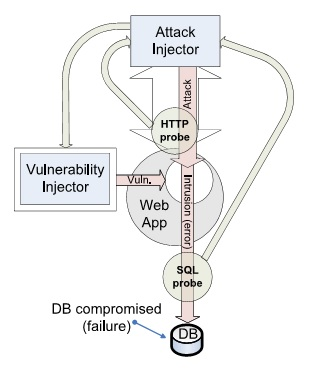
\includegraphics[scale=.8]{Main/Fig3}}
\caption{VAIT internal components}
 \label{fig:1}
\end{center}
\end{figure}

\subsection{Vulnerability Injection Stage}
 In the vulnerability injection stage, the vulnerabilities
are injected into the web application. For this purpose, it
needs information about which input variables carry relevant information that can be used to execute attacks to the web application. This stage starts by analyzing the
source code of the web application files searching for locations where vulnerabilities can be injected (Fig. 3.3). The injection of vulnerabilities is done by removing the protection of the target variables, like the call to a sanitizing
function. This process follows the realistic patterns resulting from the field study presented in [16]. Once it finds a
possible location, it performs a specific code mutation in
order to inject one vulnerability in that particular location.
The change in the code follows the rules derived from
[16], which are described and implemented as a set of
Vulnerability Operators.\\
\newline
The Vulnerability Operators are built upon a pair of
attributes: the Location Pattern and the Vulnerability Code
Change. The Location Pattern defines the conditions that
a specific vulnerability type must comply with and the
Vulnerability Code Change specifies the actions that
must be performed to inject this vulnerability, depending
on the environment where the vulnerability is going to
be injected.\\
\newline
The vulnerability and attack injection uses both
dynamic analysis and static analysis to gather the data
needed to apply the vulnerability operators. This analysis obtains not only the input variables (IV) that will be
part of an output variable (OV), but also the chain of variables in between. If the web application is secured, one
of the variables in the chain is sanitized or filtered
(Fig. 3.4). This variable is called target variable (TV),
because it is the one that the vulnerability injection stage
will try to make vulnerable by removing or changing the
protection scheme, according to the Vulnerability Operators. To inject a vulnerability using the Vulnerability
Operators, information about the target variable and the code location (CL) where it is sanitized or
filtered \{TV, CL\} is needed.
\begin{figure}
\centering
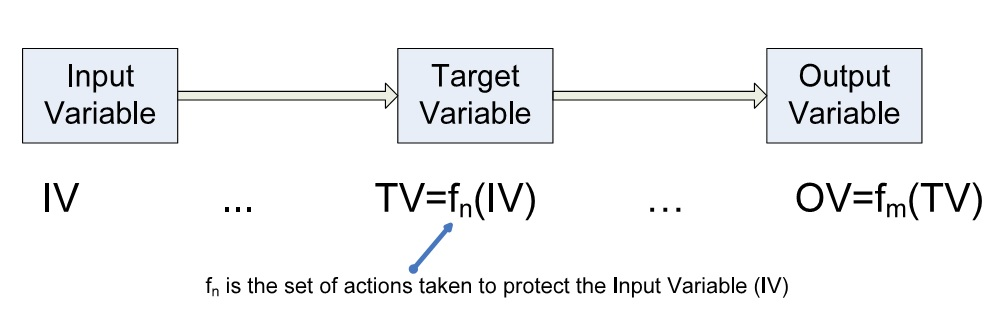
\includegraphics[width=0.7\linewidth]{Main/Fig4}
\caption{Chain of variables from input to output of the Web Application.}
\label{fig:Fig4}
\end{figure}\\
\newline
The preparation stage obtains  the pairs \{$ IV_{(dynamic analysis)}; OV_{(dynamic analysis)} $\}, which are the set of
input variables ($ IV_{(dynamic analysis)} $) whose values come from
the HTTP interaction or the SQL communication and their
mapping with output variables ($ OV_{(dynamic analysis)} $). On the other side, the vulnerability injector tool performs a static analysis on the source code and finds the input variables ($ IV_{(static analysis)} $) that are expected to be seen in the
output ($ OV_{(static analysis)} $) as part of the HTML response,
SQL queries, etc. It also provides the target variable
($ TV_{(static analysis)} $) and the code location ($ CL_{(static analysis)} $)
of the place in the file where the target variable is sanitized
or filtered. Overall, the static analysis provides the following set of attributes: \{$ IV_{(static analysis)}; OV_{(static analysis)} TV_{}(static analysis),$ \\$ CL_{(static analysis)}. $\}
%$ TV_{(static analysis); CL_{(static analysis)} $\}.
\\
\newline
The correlation of variables resulting from both static
and dynamic analysis originates a more precise set of locations where the Vulnerability Operators may be used. The
outcome of this correlation is an improved collection of
vulnerabilities that has a higher rate of exploitability by
the attack injection mechanism. The data must be provided
by the set of attributes that come from the static analysis
\{$ IV_{(static analysis)}, OV_{(static analysis)},$ \\ $ TV_{(static analysis)},
	CL_{(static analysis)} $\}, but improved by the pair of attributes
that come from the preparation stage \{$ IV_{(dynamic analysis)},
	OV_{(dynamic analysis)} $\} (Fig. 3.5). It considers the data from
the set of attributes \{$ IV_{(static analysis)}, OV_{(static analysis)},$
$TV_{(static analysis)}, $ \\ $CL_{(static analysis)} $\} but only whose pairs
\{IV$ _{}(static analysis), OV_{(static analysis)} $ \} are equivalent to any of
the \{$ IV_{(dynamic analysis)}, OV_{(dynamic analysis)} $ \}. The procedure to
process the data from dynamic and static analysis to obtain
the match outcome consisting of the pair of target variable
and code location \{TV, CL\} needed to apply the vulnerability operators
\begin{figure}
\centering
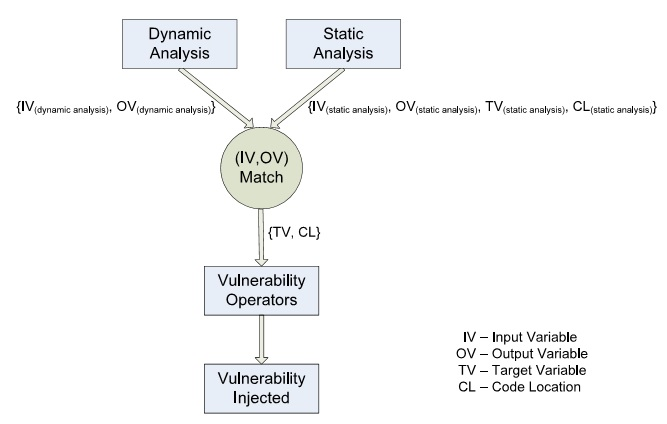
\includegraphics[width=0.7\linewidth]{Main/Fig5}
\caption{Using data from dynamic and static analysis to apply the vulnerability operators and inject a vulnerability.}
\label{fig:Fig5}
\end{figure}


\subsection{AttackLoad Generation Stage}
After having the set of copies of the web application
source code files with vulnerabilities injected, the collection of malicious interactions (attackloads) that will be used to attack each vulnerability need to be generated. This
is done in the attackload generation stage. The attackload
is the malicious activity data needed to attack a given vulnerability. This data is built around the interaction patterns derived from the preparation stage, by tweaking
the input values of the vulnerable variables.\\
\newline
The value that is assigned to the vulnerable variable, in
order to attack it, results from a fuzzing process. In this
process, the malicious value is obtained through the
manipulation of the data provided by the good values of
the vulnerable variable, the prefix $ (>,),`,``, \dots) $ and the suffix $ (<,–,\#,`,",\dots) $, the use of attackload strings and predefined functions (Fig. 3.6).The fuzzing process consists of combining the available collection of prefixes, attackload strings and suffixes.\\
\newline
\begin{figure}[H]
\centering
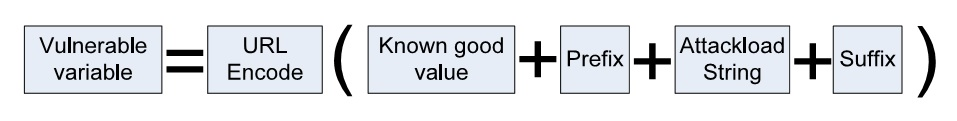
\includegraphics[width=0.7\linewidth]{Main/Fig6}
\caption{Fuzzer generated malicious variable value.}
\label{fig:Fig6}
\end{figure}
This stage also generates the payload footprints that
have a one to one relationship with the attack payloads.
The payload footprints are the expected result of the
attack. They can be the malicious SQL queries text sent to
the database, for the case of an SQLi attack; or the HTML
of the web application response, for the case of a XSS
attack. These payload footprints are fundamental, since
they are used to assess the success of the attack.

\subsection{Attack Stage}
In the attack stage, the web application is, once again, interacted. However, this time it is a ``malicious'' interaction since it consists of a collection of attack payloads in order to
exploit the vulnerabilities injected. The attack intends to
alter the SQL query sent to the database server of the web
application (for the case of SQLi attacks) or the HTML data
sent back to the user (for the case of XSS attacks).\\
\newline
The vulnerable source code files (from the vulnerability injection stage) are applied to the web application,
one at a time. Once again the two probes for capturing
the HTTP and SQL communications are deployed and
the collection of attackloads is submitted to exploit the vulnerabilities injected (Fig. 3.3). The interaction with the
web application is always done from the web client’s
point of view (the web browser) and the attackload is
applied to the input variables (the text fields, combo
boxes, etc., present in the webpage interface). At the end
of the attack, it is assessed for success. The
detection of the success of the attack is done by searching
for the presence of the payload footprint in the interaction
data (HTTP or SQL communications) captured by the two
probes. The process is repeated until all the injected vulnerabilities have been attacked.\\
\newline

\pagebreak


\section{VULNERABILITY \& ATTACK INJECTOR TOOL}

To demonstrate the feasibility of the proposed attack injection methodology, a prototype tool is developed ; Vulnerability \& Attack Injector Tool (VAIT).The VAIT prototype targets Linux, Apache, MySQL and PHP web applications, which is currently one of the most commonly used solution stack to develop web applications.\\
\newline
VAIT can injects vulnerabilities into the web application code and attacks them
in a seamlessly manner. As explained earlier, the process of attacking the web application
consists of 4 stages: the preparation stage, the vulnerability
injection stage, the attackload generation stage and the attack
stage (Fig 3.7). All this vulnerability and attack injection process will
be done with minimum human intervention.  The VAIT is
configured with the web application folder location. Then
the preparation stage is executed while the web application is being interacted. At the end, the vulnerability
injection stage automatically generates the vulnerabilities,
followed by the attackload generation stage that generates the attack payloads. At this point, the attack stage
can be executed to attack the vulnerabilities, collect the
results and calculate the attack success.
\begin{figure}
\centering
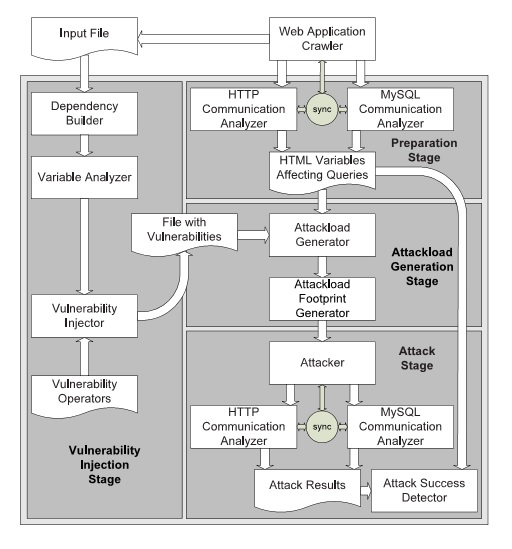
\includegraphics[width=0.7\linewidth]{Main/fig7}
\caption{VAIT architecture.}
\label{fig:fig7}
\end{figure}\\
\newline
During the preparation stage, the web application is executed. This interaction can be made either manually, by someone executing every web application procedure that should be tested, or automatically using an external tool, such as a web application crawler. During this interaction, the VAIT monitors the HTTP communication between the web browser and the web server and all the SQL communications going to and from the database server.\\
\newline
Monitoring is implemented using built-in proxies specifically developed for the HTTP and for the SQL communications. These proxies send a copy of the entire packet data
traversing them through the configured socket ports to the
HTTP Communication Analyzer and MySQL Communication
Analyzer components. Proxies run as independent processes
and threads, so they are relatively autonomous. To guarantee synchronization with other components of the VAIT, a
Sync mechanism was also built-in (Fig.3.7). The synchronism
is obtained by executing each web application interaction in
sequence without overlapping (i.e., without the common
use of simultaneous threads to speedup the process) and
gathering the precise time stamps of both the HTTP communication and respective SQL query. The interaction starts with the client actor (the browser of
the user of the web application) sending one HTTP request
that may lead SQL query requests to be sent to the database
server. Next, the database server responds to the SQL query
requests and sends the response back to the web application
server. Finally, the application server sends the HTTP
response back to the client actor. When the HTTP and SQL
proxies capture these serialized operations they also register
their time stamps, which allows the Sync mechanism to
group this distributed set of actions into meaningful causeeffect sequences.\\
\newline
The information gathered by both proxies contains the
structure of each webpage, the associated input variables, typical values and the associated SQL queries
where these variables are used. During this interaction,
the list of the web application files that are being run is
also sent to the integrated Vulnerability Injector as input
files. The vulnerability injector component is executed for each one, delivering the respective group of files with
injected vulnerabilities.\\
\newline
%\pagebreak
%\section{PROPOSED METHOD}
The current paper detects only the SQL injection(SQLi) attack and Cross Site Scripting (XSS) attacks. These two are the most common vulnerability found in the web application world.These two attacks attack the application data and the user information available with the system.But there are some other forms of attacks, targeting the server machine which runs these application itself.Attacks like Remote Code Execution (RCE) and File Inclusion (FI) attacks target the vulnerability in the web application and attacks the server machine instead of the web application. These kinds of attack can not only cause damage to the web application, but can even trouble the entire applications and services running on the main hardware and can even damage the normal working of the server operating system.\\
\newline
The VAIT tool proposed in the paper can be extended in order to identify the Remote Code Execution (RCE) and File Inclusion (FI) attack.Since these attacks does not necessarily need to have a communication with database, the attack cannot be identified by analyzing HTTP proxies and SQL proxies.Hence to identify these kinds of attack other methods have to be utilized.Static code analysis can identify these kinds of vulnerabilities easily but is very ineffective due to high false positive rates and low precision. One of the common way to identify these attacks are by analyzing the http data packets and performing a pattern matching analysis in it in order to identify erroneous patter.\\
\newline
A pattern mining approach based on dynamic analysis on input data and available information on method execution can easily identify attack injections of these kinds.So by utilizing a pattern mining algorithm and integrating it with the VAIT tool, the web application evaluation capability of the tool will be extended .





%\chapter{EXPERIMENTAL RESULTS AND ANALYSIS}\label{chp:chapter4}
\thispagestyle{fancy}

\chapter{CONCLUSION}\label{chp:chapter5}
\thispagestyle{fancy}
The paper proposes a  methodology to automatically
inject realistic attacks in web applications. This methodology consists of analyzing the web application and generating a set of potential vulnerabilities. Each vulnerability is
then injected and various attacks are mounted over each
one. The attack injection consists of the introduction of realistic vulnerabilities that are afterwards automatically exploited. The success of each attack is automatically assessed
and reported.To understand the feasibility of the method an attack injection tool VAIT is proposed which will try to automate the process with less human effort.
The proposed tool can highlight and overcomes implementation specific issues.The system emphasized the need to match the results of the dynamic and the static analysis of the web applications.The toll will uses Linux, Apache, MySQL and Php for the evaluation purpose.
The VAIT tool can be used as a practical environment that can be used to test
counter measure mechanisms (such as IDS, web application vulnerability scanners, firewalls, etc.), train and evaluate security teams, estimate security measures.


\begin{thebibliography}{8}
\addcontentsline{toc}{chapter}{\bf BIBLIOGRAPHY}

\bibitem{1}
cgisecurity.net, www.cgisecurity.com/articles/csrf-faq.shtml\#
whatis, Dec. 2008.

\bibitem{2}
G. Alvarez and S. Petrovic,  ``A New Taxonomy of Web Attacks Suitable for Efficient Encoding,'' Computers and Security, vol. 22,
no. 5, pp. 435-449, July 2003

%H. Chang, D.-Y. Yeung, and Y. Xiong,  ``Super-resolution through neigh-
%bor embedding,'' in Proc. IEEE Conf. Comput. Vis. Pattern Recognit.,
%Jul. 2004, pp. 275–282.


\bibitem{3}
S. Christey and R. Martin,  ``Vulnerability Type Distributions in
CVE,'' Mitre Report, May 2007.

\bibitem{4}
J. Duraes and H. Madeira,  ``Emulation of Software Faults: A Field
Data Study and a Practical Approach,'' IEEE Trans. Software Eng.,
vol. 32, no. 11, pp. 849-867, Nov. 2006.

\bibitem{5}
M.R. Lyu, Handbook of Software Reliability Engineering. IEEE
Computer Society Press \& McGraw-Hill, 1996.

\bibitem{6}
J. Williams and D. Wichers,  ``OWASP Top 10,'' OWASP Foundation, Feb. 2013.

\bibitem{7}
N. Neves, J. Antunes, M. Correia, P. Verissimo, and R. Neves,
 ``Using Attack Injection to Discover New Vulnerabilities,'' Proc.
IEEE/IFIP Int’l Conf. Dependable Systems and Networks, 2006.

\bibitem{8}
J. Fonseca, M. Vieira, and H. Madeira,  ``Testing and Comparing
Web Vulnerability Scanning Tools for SQLi and XSS Attacks,''
Proc. IEEE Pacific Rim Int’l Symp. Dependable Computing, Dec. 2007.

\bibitem{9}
S. Clowes,  ``A Study in Scarlet, Exploiting Common Vulnerabilities in PHP Applications,'' http://www.securereality.com.au/
studyinscarlet.txt, 2013.

\bibitem{10}
B. Livshits and S. Lam,  ``Finding Security Vulnerabilities in Java
Applications with Static Analysis,'' Proc. USENIX Security Symp.,
pp. 18-18, 2005.

\bibitem{11}
M. Buchler, J. Oudinet, and A. Pretschner,  ``Semi-Automatic Security Testing of Web Applications from a Secure Model,'' Proc. Int’l
Conf. Software Security and Reliability, 2012.

\bibitem{12}
S. McConnell, ``Gauging Software Readiness with Defect
Tracking'', IEEE Software, vol. 14, no. 3, May/June 1997.

\bibitem{13}
N. Nagappan, L. Williams, J. Hudepohl, W. Snipes, M. Vouk,
 ``Preliminary Results on Using Static Analysis Tools for Software
Inspection.'' Proc. Int’l Symp. Software Reliability Eng., pp. 429-439,
2004.
\bibitem{14}
OSVDB,  ``Open Sourced Vulnerability Database,'' http://osvdb.
org, May 2013.
\bibitem{15}
D. Powell and R. Stroud,  ``Conceptual Model and Architecture of
MAFTIA,'' Project MAFTIA, Deliverable D21, 2003.

\bibitem{16}
J. Fonseca and M. Vieira,  ``Mapping Software Faults with Web
Security Vulnerabilities,'' Proc. IEEE/IFIP Int’l. Conf. Dependable
Systems and Networks, June 2008

\bibitem{17}
S. Fogie, J. Grossman, R. Hansen, A. Rager, and P. Pektov, XSS
Attacks: Cross Site Scripting Exploits and Defense. Syngress, 2007.
Intell., vol. 32, no. 6, pp. 1127–1133, Jun. 2010.
\bibitem{18}
J. Arlat, A. Costes, Y. Crouzet, J.-C. Laprie, and D. Powell,  ``Fault
Injection and Dependability Evaluation of Fault-Tolerant Systems,'' IEEE Trans. Computers, vol. 42, no. 8, pp. 913-923, Aug.
1993.
\bibitem{19}
T. Scholte et al.,  ``An Empirical Analysis of Input Validation
Mechanisms,'' Proc. ACM Symp. Applied Computing, pp. 1419-1426,
2012.

\bibitem{20}
J. Carreira, H. Madeira, and J.G. Silva,  ``Xception: Software Fault
Injection and Monitoring in Processor Functional Units,'' IEEE
Trans. Software Eng., vol. 24, no. 2, Feb. 1998.

\bibitem{21}
 N. Tomatis, R. Brega, G. Rivera, and R. Siegwart,  ``May You Have
 a Strong (-Typed) Foundation’ Why Strong Typed Programming
 Languages Do Matter,'' Proc. IEEE Int’l Conf. Robotics and
 Automation, 2004.
 
\bibitem{22}
J. Christmansson and R. Chillarege,  ``Generation of an Error Set
that Emulates Software Faults,'' Proc. IEEE Fault Tolerant Computing Symp., 1996.
\bibitem{23}
H Madeira, M. Vieira, and D. Costa,  ``On the Emulation of Software Faults by Software Fault Injection,'' Proc. IEEE/IFIP Int‘l
Conf. Dependable System and Networks, 2000.

\bibitem{24}
M. Cukier, R. Berthier, S. Panjwani, and S. Tan,  ``A Statistical
Analysis of Attack Data to Separate Attacks,'' Proc. Int’l Conf.
Dependable Systems and Networks, pp. 383-392, 2006.

\end{thebibliography}
\end{document}
